\documentclass{article}
 \usepackage[spanish]{babel}
 \usepackage{amsmath,amssymb}
\usepackage[amssymb]{SIunits}
%\usepackage{enumerate}
% \usepackage{lipsum}
% \usepackage{natbib}
\usepackage{graphicx}
\usepackage{analysis_orax}
\usepackage{subcaption}
\usepackage{hyperref}
\usepackage{listings}
\usepackage{marvosym}

\title{Escritura de documentos científicos}

\author{Diego Restrepo\footnote{\href{mailto:restrepo@udea.edu.co}{restrepo@udea.edu.co}}\\
\textit{\small  Instituto de Física, Universidad de Antioquia}
}
\date{\small Octubre 13, 2017}
\begin{document}
\maketitle

\begin{abstract}
En la edición de textos de documentos que requieran algún formato
especial, siempre se recomiendo enfocarse en el contenido de los textos y
dejar que el formato se realice de forma automática. \LaTeX{} esta especialmente diseñado para ese fin, aún en el caso de textos sin matemáticas.
\end{abstract}
\section{Aclaración}
Una vez recibido este documento por favor cree una copia del mismo para futura referencia y trabaje directamente sobre este documento borrando todos los contenidos del mismo. Esto con el fin de poder activar el sistema automático de revisión que requiere una cuenta especial desde la cual el presente documento fue creado. 
\section{Documentos estructurados}
Los documentos científicos están diseñados pensando más en un documento de tipo impreso que en una página web. La principal diferencia en este aspecto es la optimización del uso y el espacio del papel para garantizar una lectura cómoda. Los algoritmos de \LaTeX{} están optimizados para este tipo de usos. Las letras y palabras de distribuyen de la forma más óptima posible tanto horizontal como verticalmente. Una técnica básica de los documentos impresos que chocan frontalmente con los documentos electrónicos es la separación de los párrafos. En los documentos escritos la única separación entre los párrafos es la sangría al comienzo de la línea que indica la diferencia entre un punto seguido, como el punto inmediatamente anterior en esté párrafo, del siguiente punto y aparte:  $\cdots$ \hfill éste es un punto aparte.

En el párrafo anterior se ha forzado que la última palabra antes del punto aparte quede justo al final de la línea para maximizar el efecto de la sangría, la  cual consiste en unos espacios en blanco justo antes del comienzo del nuevo párrafo. La separación de párrafos en LaTeX ocurre de forma natural simplemente dejando una línea en blanco entre ellos. 

Como recomendación general, ya sea que se use un procesador de palabras o un editor de texto plano, se debe evitar forzar el formato. Por ejemplo, si va a escribir el título de una sección numerada, debe evitar poner manualmente los atributos del texto como números, el formato en negrilla, o el tamaño de la letra. Si se esta en un procesador de texto debe usar las definiciones de estilo apropiadas, mientras que si esta trabajando en un editor de texto plano, debe usar los comandos de estructura del programa específico de generación del documento formateado. En el último caso se recomienda, siempre que sea posible, usar los comandos de estilo en lugar de los comandos de formateo del texto:

Es así como en \LaTeX{} podemos establecer una sección de un documento tipo artículo como:
\begin{lstlisting}
\section{Hola mundo}
\end{lstlisting}
que produce el resultado:

%\begin{minipage}
\noindent \textbf{\large 1 Hola mundo}\\
%\begin{minipage}
¡Y ésta es la opción recomendada!     

Forzar el formato corresponde a obtener lo mismo usando comandos de formato como:
\begin{lstlisting}
\textbf{\large 1 Hola mundo}
\end{lstlisting}
que en principio da el mismo el resultado:

\noindent \textbf{\large 1 Hola mundo}\\
Sin embargo, se debe evitar este tipo de formato manual.

A continuación se establecen algunas de las ventajas de la estructuración de documentos
  \begin{itemize}
  \item   Marcación descriptiva versus marcación procedimental.
  \item   El autor se centra en la labor de escritura y creación, sin distraerse con asuntos que no son relevantes en el proceso de autoría.
  \item  El documento es independiente de la plataforma, facilitando su manejo, almacenado, consulta y procesado.
  \item   Sencillez de edición y fácil manejo con cualquier clase de herramientas de edición de textos.
  \item   Apoyado por un adecuado sistema de representación, mejora la calidad final de los documentos y unifica el uso de las convenciones de estilo de cada idioma y área de conocimiento.
  \item   Gracias al riguroso diseño también se facilita la automatización del proceso y el intercambio de documentos por medios informáticos. 
  \end{itemize}
  
\section{Escritura de textos científicos}  
Hay varios aspectos a tener en cuenta a la hora de escribir textos científicos. La recomendación principal es escribir ideas cortas (de no más de dos o tres líneas) separadas de puntos seguidos. Otra recomendación importante es no intentar forzar el formato del documento, permitiendo que \LaTeX\ haga su trabajo.

En particular los párrafos deben quedar separados por un punto aparte y continuación una sangría.%, es decir unos espacios en blanco antes de la nueva línea. 
Esto se consigue en \LaTeX\ automáticamente al separar los párrafos con una o más líneas. El uso del comando de ruptura de línea: \verb|\\|, debe evitarse a toda costa, y sólo debe usarse en los casos realmente necesarios.  


Las ecuaciones centradas hacen parte del párrafo y deben llevar los signos de puntuación apropiados. Se recomienda dejar un espacio pequeño, del tipo \verb|\,| antes del signo de puntuación de la ecuación, cuando la ecuación no termine en paréntesis u otros signos de agrupación. Por ejemplo:
\begin{lstlisting}
El siguiente párrafo contiene la siguiente ecuación
\begin{equation}
  \label{eq:1}
  y=x\,,
\end{equation}
la cual se sigue discutiendo aquí.

Y este es un nuevo párrafo.
\end{lstlisting}
El resultado es:

El siguiente párrafo contiene la siguiente ecuación
\begin{equation}
  \label{eq:1}
  y=x\,,
\end{equation}
la cual se sigue discutiendo aquí.

Y este es un nuevo párrafo.

\bigskip

Note que no hay líneas en blanco ni antes del \verb|\begin{equation}|, ni después del \verb|\end{equation}|. Si la ecuación termina en un punto aparte, entonces se debe dejar una línea en blanco después del \verb|\end{equation}| para iniciar el nuevo párrafo:

\begin{lstlisting}
Este  párrafo termina con la siguiente ecuación
\begin{equation}
  \label{eq:bin}
  x^2-y^2=(x-y)(x+y).
\end{equation}

Y este es un nuevo párrafo.
\end{lstlisting}
El resultado es:

Este  párrafo termina con la siguiente ecuación
\begin{equation}
  \label{eq:bin}
  x^2-y^2=(x-y)(x+y).
\end{equation}

Y este es un nuevo párrafo. 

La referencia a una ecuación siempre se debe hacer usando el sistema de refencias cruzadas de \LaTeX{}. A la ecuación a referenciar se le debe asignar un rótulo usando el comando \verb|\label| ilustrado en la ecuación anterior. Para referirse a ella dentro del texto se usa el comando \verb|\eqref| con el correspondiente rótulo asignado, que da lugar a la ecuación~\eqref{eq:bin}, obtenida con \verb|\eqref{eq:bin}|. Se recomiendo siempre poner un identificador al rótulo, en el caso anterior es \verb|eq:|, el cual indica un rótulo de ecuación.

\subsection{Modo texto y modo matemático}

El modo texto y el modo matemático usan diferentes estilos de texto para facilitar la lectura y evitar confusiones. Esto se consigue automáticamente en \LaTeX\ usando siempre los ambientes de ecuaciones centradas tipo \verb|equation| para ecuaciones de una sola línea, o \verb|align| para ecuaciones de varías líneas. 
\footnote{\texttt{align} funciona para todo tipo de ecuaciones centradas y por consiguiente reemplaza el uso de \texttt{equation}. }
Ver un tutorial de AMS-\LaTeX\ para los detalles correspondientes. Para \emph{cualquier} expresión matemática se debe encerrar  \emph{siempre} la expresión matemática entre símbolos de \verb|$...$|.
Esto se debe hacer incluso en el caso de variables de una sóla letra, tipo $a$ o $x$. Es decir, usando: \verb|$a$| o \verb|$x$|.

Para usar modo texto dentro de modo matemático se recomienda el uso del comando \verb|\text{...}|. En particular, las unidades siempre deben ir en modo texto!. Por ejemplo $1\ \text{s}$, que se obtiene con \verb|$1\ \text{s}$|. Note que la unidad está separada de la cantidad con un espacio en blanco: '\verb|\ |'. Cualquier palabra o acrónimo dentro de una ecuación debe ir en formato texto. Por ejemplo, la longitud de un alambre blanco (AB) se podría denotar con $L_{\text{AB}}$: \verb|L_{\text{AB}}|, mientras que $L_{AB}$: \verb|L_{AB}|, podría ser una matriz con índices $A$ y $B$.

Finalmente, los nombres de las funciones deben ir siempre en modo texto y con el espacio adecuado después del nombre de la función. Esto se consigue automáticamente usando los macros de funciones de \LaTeX\ del tipo: \verb|\sin|, \verb|\cos|, \verb|\exp|, etc. Por ejemplo $x=\exp(\log(x))$  que se consigue con \verb|$x=\exp(\log(x))$|. Si una función no tiene un macro de \LaTeX{} asociado, se puede usar el comando genérico \verb|\operatorname|, como en  $x=\operatorname{e}^{\log x}$: \verb|$x=\operatorname{e}^{\log x}$|.


\subsection{Objetos flotantes}

Las tablas y figuras se suelen poner como elementos flotantes en el documento con algún texto explicativo: \verb|\caption{}|. Para el caso de la figura~\ref{fig:detector} se uso:

\begin{lstlisting}
\begin{figure}
    \centering
    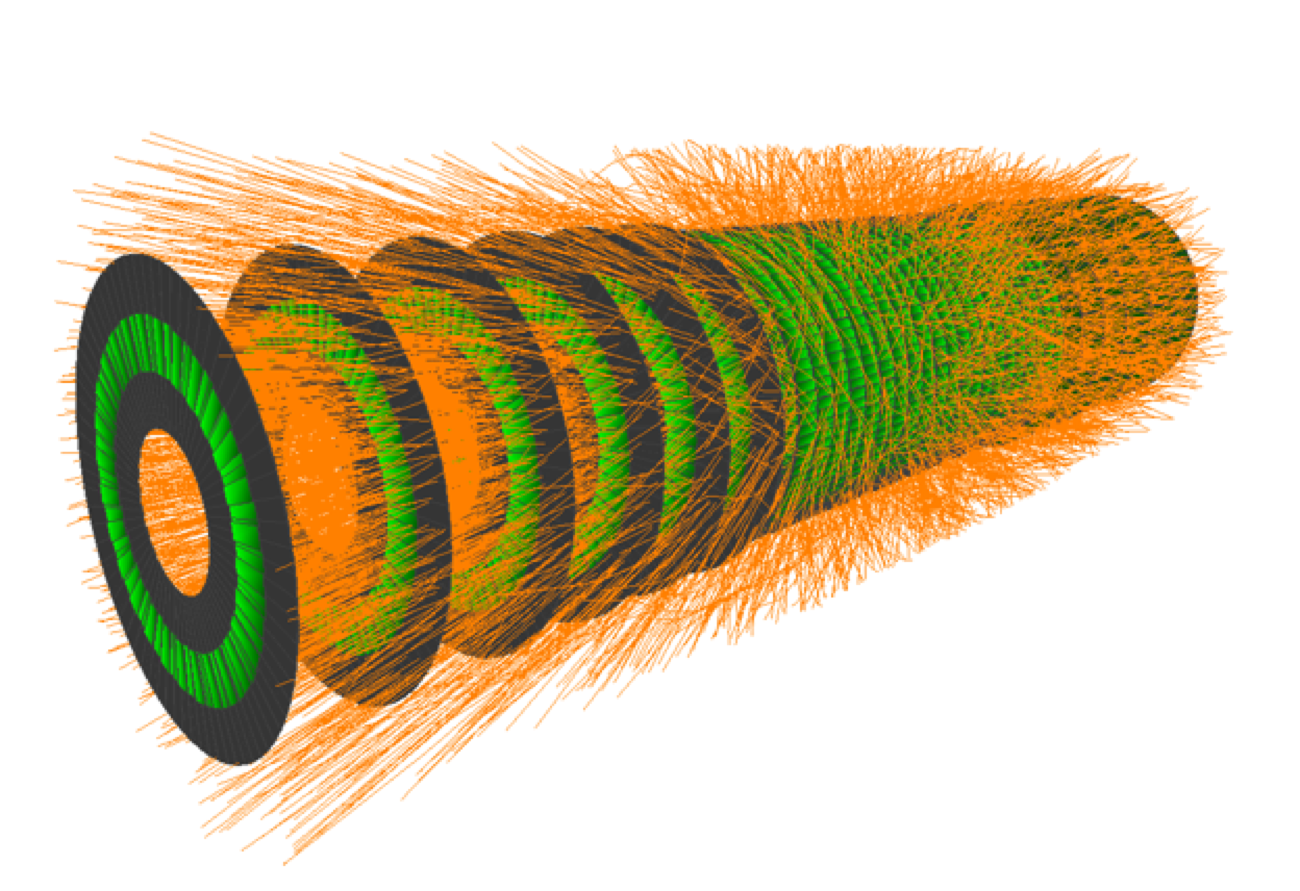
\includegraphics[scale=0.2]{figures/cern_graphic}
    \caption{Ilustración de la geometría de los detectores}
    \label{fig:detector}
\end{figure}
\end{lstlisting}


Por lo tanto siempre deben ser referenciadas cuando se discutan dentro del texto, como se ilustra en la figura \ref{fig:detector}. Esto se logra usando el sistema de referencias cruzadas de \LaTeX{} con \verb|\label| y \verb|\ref|. \LaTeX{} determina automáticamente la posición de la figura dentro del texto y como está referenciada no importa que no aparezca inmediatamente después del párrafo donde se referencia. En lo posible las figuras deben ser de tipo vectorial, en formato PDF, para garantizar que escalen bien con cualquier magnificación del documento. 

\begin{figure}
    \centering
    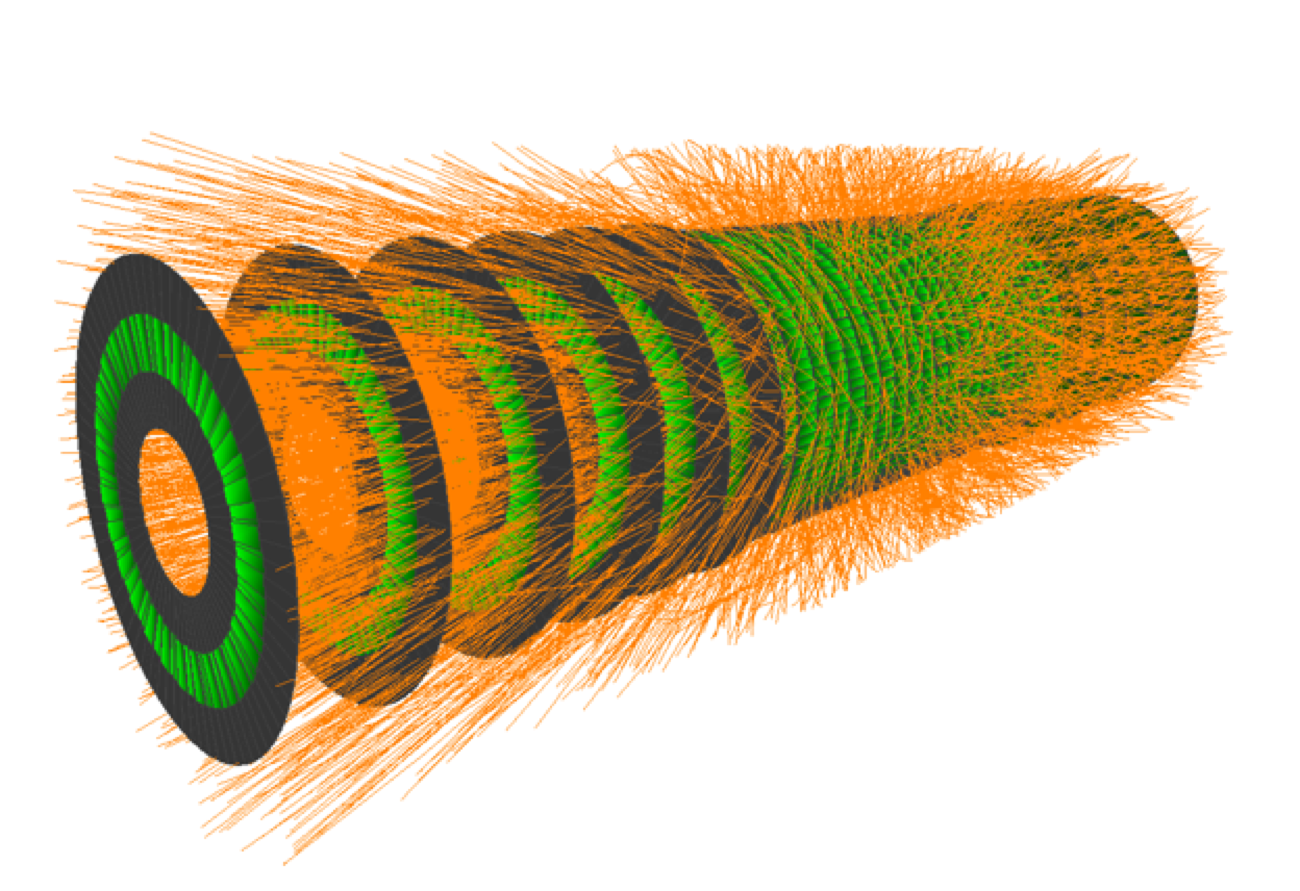
\includegraphics[scale=0.2]{figures/cern_graphic}
    \caption{Ilustración de la geometría de los detectores}
    \label{fig:detector}
\end{figure}

\section{Recomendaciones finales}
\begin{itemize}
\item Organizar los espacios entre ecuaciones y texto entre diferentes párrafos.
\item Realizar la debida puntuación entre ecuaciones y
texto para lograr una lectura más fluida. Buscar sinónimos de expresiones
y verbos conectores para evitar repeticiones dentro del párrafo. A su vez, comprobar
la conjugación uniforme de tiempos verbales.
\item Identificar las frases que resulten largas y complicadas de
leer y separarlas en frases de menor extensión manteniendo el significado
y contenido de la mismas.
\end{itemize}

\section{Referencias bibliográficas}
El sistema de referencias bibliográficas de \LaTeX\ también se basa en rótulos definidos en la bibliografía que son llamados desde el texto con el comando  \verb|\cite|. En el caso de este documento, se usa el sistema BibTeX que se basa en un archivo externo con extensión \verb|.bib|, el cual hemos llamado \verb|susy.bib|. Este archivo  se carga con el comando \verb|\bibliography|. Para que este archivo pueda ser procesado, se requiere un archivo con extensión \verb|.bst|  con las instrucciones correspondientes para generar la entrada bibliográfica. En nuestro caso dicho  archivo corresponde al \verb|apsrev4-1long.bst| el cual se carga con el comando \verb|\bibliographystyle|.
El comando \verb|bibtex| extrae las referencias necesarias del archivo \verb|.bib| para generar un archivo \LaTeX\ de referencias bibliográficas con extensión \verb|.bbl| de acuerdo a las reglas de estilo del archivo \verb|.bst|.

Para que todo esto ocurra, al final del documento se deben adicionar las siguientes líneas 
\begin{lstlisting}
\bibliographystyle{apsrev4-1long}
\bibliography{susy}
\end{lstlisting}
y durante la compilación, después de ejecutar el comando de \LaTeX, se debe ejecutar el comando \verb|bibtex|, antes de correr el comando de \LaTeX\ de nuevo. Desde la consola de Linux, para compilar un archivo \verb|documento.tex|, la secuencia de comandos debe ser:
\begin{lstlisting}
$ pdflatex documento 
$ bibtex documento
$ pdflatex documento 
$ pdflatex documento 
\end{lstlisting}
Estos comandos son realizados automáticamente en las plataformas de \LaTeX\ online como Overleaf o ShareLaTeX. 
Es de anotar que el documento creado con extensión \verb|.bbl| contiene toda la información de las referencias usadas en el documento y es el usualmente requerido por las revistas para su proceso interno de edición. Esto se debe a que la base de datos  bibliográfica (\verb|susy.bib| en nuestro caso)  puede ser reutilizada en otros documentos y por lo tanto termina teniendo muchas más referencias de las que realmente se necesitan en el documento específico.

De este modo, una referencias del tipo: \verb|\cite{Bernal:2015bla}|, cuyo rótulo \verb|Bernal:2015bla| está definido en el archivo \verb|susy.bib|, aparece en el texto de la siguiente manera: \cite{Bernal:2015bla}. Además se genera una sección adicional del documento con la descripción de la referencia correspondiente. Es altamente recomendable obtener las referencias bibliográficas (BibTeX en este caso) desde algún sistema de manejo de referencias para facilitar el proceso de extracción automático de referencias por parte de terceros. En nuestro caso la referencia la obtuvimos desde \href{http://inspirehep.net/record/1338091/export/hx}{\texttt{http://inspire.hep}}. Una vez allí copiamos y pegamos el texto correspondiente:
\begin{footnotesize}
\begin{lstlisting}
@article{Bernal:2015bla,
      author         = "Bernal, Nicolas and Garcia-Cely, Camilo and Rosenfeld,
                        Rogerio",
      title          = "{WIMP and SIMP Dark Matter from the Spontaneous Breaking
                        of a Global Group}",
      journal        = "JCAP",
      volume         = "1504",
      year           = "2015",
      number         = "04",
      pages          = "012",
      doi            = "10.1088/1475-7516/2015/04/012",
      eprint         = "1501.01973",
      archivePrefix  = "arXiv",
      primaryClass   = "hep-ph",
      SLACcitation   = "%%CITATION = ARXIV:1501.01973;%%"
}
\end{lstlisting}
\end{footnotesize}
al archivo  \verb|susy.bib|. Así todo queda de acuerdo a los estándares de publicación del área correspondiente. En este caso a los estándares de la revista  Physical Review de la American Physical Society  (APS).

\bibliographystyle{apsrev4-1long}
\bibliography{susy}


\end{document}
